% Options for packages loaded elsewhere
\PassOptionsToPackage{unicode}{hyperref}
\PassOptionsToPackage{hyphens}{url}
%
\documentclass[
  ignorenonframetext,
  aspectratio=169,
]{beamer}
\usepackage{pgfpages}
\setbeamertemplate{caption}[numbered]
\setbeamertemplate{caption label separator}{: }
\setbeamercolor{caption name}{fg=normal text.fg}
\beamertemplatenavigationsymbolsempty
% Prevent slide breaks in the middle of a paragraph
\widowpenalties 1 10000
\raggedbottom
\setbeamertemplate{part page}{
  \centering
  \begin{beamercolorbox}[sep=16pt,center]{part title}
    \usebeamerfont{part title}\insertpart\par
  \end{beamercolorbox}
}
\setbeamertemplate{section page}{
  \centering
  \begin{beamercolorbox}[sep=12pt,center]{part title}
    \usebeamerfont{section title}\insertsection\par
  \end{beamercolorbox}
}
\setbeamertemplate{subsection page}{
  \centering
  \begin{beamercolorbox}[sep=8pt,center]{part title}
    \usebeamerfont{subsection title}\insertsubsection\par
  \end{beamercolorbox}
}
\AtBeginPart{
  \frame{\partpage}
}
\AtBeginSection{
  \ifbibliography
  \else
    \frame{\sectionpage}
  \fi
}
\AtBeginSubsection{
  \frame{\subsectionpage}
}
\usepackage{amsmath,amssymb}
\usepackage{iftex}
\ifPDFTeX
  \usepackage[T1]{fontenc}
  \usepackage[utf8]{inputenc}
  \usepackage{textcomp} % provide euro and other symbols
\else % if luatex or xetex
  \usepackage{unicode-math} % this also loads fontspec
  \defaultfontfeatures{Scale=MatchLowercase}
  \defaultfontfeatures[\rmfamily]{Ligatures=TeX,Scale=1}
\fi
\usepackage{lmodern}
\ifPDFTeX\else
  % xetex/luatex font selection
\fi
% Use upquote if available, for straight quotes in verbatim environments
\IfFileExists{upquote.sty}{\usepackage{upquote}}{}
\IfFileExists{microtype.sty}{% use microtype if available
  \usepackage[]{microtype}
  \UseMicrotypeSet[protrusion]{basicmath} % disable protrusion for tt fonts
}{}
\makeatletter
\@ifundefined{KOMAClassName}{% if non-KOMA class
  \IfFileExists{parskip.sty}{%
    \usepackage{parskip}
  }{% else
    \setlength{\parindent}{0pt}
    \setlength{\parskip}{6pt plus 2pt minus 1pt}}
}{% if KOMA class
  \KOMAoptions{parskip=half}}
\makeatother
\usepackage{xcolor}
\newif\ifbibliography
\setlength{\emergencystretch}{3em} % prevent overfull lines
\providecommand{\tightlist}{%
  \setlength{\itemsep}{0pt}\setlength{\parskip}{0pt}}
\setcounter{secnumdepth}{-\maxdimen} % remove section numbering
\newlength{\cslhangindent}
\setlength{\cslhangindent}{1.5em}
\newlength{\csllabelwidth}
\setlength{\csllabelwidth}{3em}
\newlength{\cslentryspacingunit} % times entry-spacing
\setlength{\cslentryspacingunit}{\parskip}
\newenvironment{CSLReferences}[2] % #1 hanging-ident, #2 entry spacing
 {% don't indent paragraphs
  \setlength{\parindent}{0pt}
  % turn on hanging indent if param 1 is 1
  \ifodd #1
  \let\oldpar\par
  \def\par{\hangindent=\cslhangindent\oldpar}
  \fi
  % set entry spacing
  \setlength{\parskip}{#2\cslentryspacingunit}
 }%
 {}
\usepackage{calc}
\newcommand{\CSLBlock}[1]{#1\hfill\break}
\newcommand{\CSLLeftMargin}[1]{\parbox[t]{\csllabelwidth}{#1}}
\newcommand{\CSLRightInline}[1]{\parbox[t]{\linewidth - \csllabelwidth}{#1}\break}
\newcommand{\CSLIndent}[1]{\hspace{\cslhangindent}#1}
\usepackage{amsmath}
\usepackage{graphicx}
\usepackage{booktabs}
\usepackage{setspace}
\usepackage{float}
\usepackage{hyperref}
\setbeamersize{text margin left=0.25in, text margin right=0.25in}
\ifLuaTeX
  \usepackage{selnolig}  % disable illegal ligatures
\fi
\IfFileExists{bookmark.sty}{\usepackage{bookmark}}{\usepackage{hyperref}}
\IfFileExists{xurl.sty}{\usepackage{xurl}}{} % add URL line breaks if available
\urlstyle{same}
\hypersetup{
  pdftitle={Effect sizes for paired data should use the change score variability rather than the pre-test variability:  A Paper by Dr.~Scott Dankel and Dr.~Jeremy P. Loenneke},
  pdfauthor={Alex Gould},
  hidelinks,
  pdfcreator={LaTeX via pandoc}}

\title{Effect sizes for paired data should use the change score
variability rather than the pre-test variability:\\
\strut \\
A Paper by Dr.~Scott Dankel and Dr.~Jeremy P. Loenneke}
\author{Alex Gould}
\date{2024-10-04}

\begin{document}
\frame{\titlepage}

\begin{frame}{Full Citation}
\protect\hypertarget{full-citation}{}
Dankel, SJ and Loenneke, JP. Effect sizes for paired data should use the
change score variability rather than the pre-test variability. J
Strength Cond Res 35(6): 1773--1778, 2021---\}
\end{frame}

\begin{frame}{What is effect size}
\protect\hypertarget{what-is-effect-size}{}
\begin{itemize}
\tightlist
\item
  Variable that provides an overall measure for magnitude of change
  (Dankel and Loenneke (2021))
\item
  Differs from a T-statistic because sample size is not included
\item
  Quantifies how much the mean of the post-treatment differs from the
  mean of the baseline score in terms of a certain standard deviation.

  \begin{itemize}
  \tightlist
  \item
    Specifically, they are looking at this comparison from the lens of
    meta-analyses for exercise science and sports medicine
  \end{itemize}
\end{itemize}
\end{frame}

\begin{frame}{Authors' Aims}
\protect\hypertarget{authors-aims}{}
\begin{itemize}
\tightlist
\item
  To convince the audience through analysis that baseline and post-test
  standard deviations (study sample measures of variability) don't tell
  the full story on the overall variability of the intervention.
\item
  To convince the readers that the heterogeneity of the study sample can
  play a part in unintentionally influencing effect size measurements.
\end{itemize}

How would one describe the two types of aforementioned variability?
\end{frame}

\begin{frame}{Variability of the Study Sample}
\protect\hypertarget{variability-of-the-study-sample}{}
\begin{itemize}
\tightlist
\item
  Any measure of difference between subjects in a given treatment group
\item
  Represented by the Baseline and Post-treatment Standard Deviation.
\item
  Dankel and Loenneke (2021) and his team claim that the use of this
  type of variability in paired-sample studies is useless as it has
  nothing to do with the treatment itself
\end{itemize}
\end{frame}

\begin{frame}{Variability of the Intervention}
\protect\hypertarget{variability-of-the-intervention}{}
\begin{itemize}
\tightlist
\item
  Any measure of difference between baseline and post-treatment measure
\item
  Represented in this case by the Standard Deviation of Change Scores (I
  will elaborate on this later)
\item
  Dankel and his team prefer this method of assessing variability
\end{itemize}
\end{frame}

\begin{frame}{Dr.~Scott Dankel}
\protect\hypertarget{dr.-scott-dankel}{}
\begin{itemize}
\tightlist
\item
  Professor at Rowan University, a public research university in New
  Jersey
\item
  Attended the University of Mississippi to pursue a Masters and PhD in
  Exercise Science
\item
  Research Interests include acute and chronic adaptations to blood flow
  restricted exercise (Lab 2024)
\end{itemize}
\end{frame}

\begin{frame}{Dr.~Jeremy Paul Loenneke}
\protect\hypertarget{dr.-jeremy-paul-loenneke}{}
\begin{itemize}
\item
  Professor at The University of Mississippi
\item
  Attended Southeast Missouri State for his Bachelors and Masters in
  Nutrition and Exercise Science
\item
  Eventually got his PhD in Exercise Physiology at the University of
  Oklahoma
\item
  Research Discipline is in Skeletal Muscle Plasticity (Ole Miss 2024)
\item
  Regarding the disciplines of the authors, this paper was published in
  The Journal of Strength and Conditioning Research. This is a good
  example of the use of statistics as an interdisciplinary tool
\end{itemize}
\end{frame}

\begin{frame}{Introduction}
\protect\hypertarget{introduction}{}
\begin{block}{Specific Effect Size Measures}
\protect\hypertarget{specific-effect-size-measures}{}
The author's claim that the common effect size measures listed below are
used exhaustively in meta-analyses in the exercise science discipline.

\begin{itemize}
\item
  Cohen's d (Cite)
\item
  Hedge's g (Cite)
\item
  Glass delta (Cite)
\item
  Each use some combination of baseline standard deviation and
  post-treatment standard deviation.
\item
  Measures of variability of the study sample
\end{itemize}
\end{block}
\end{frame}

\begin{frame}{Paired Data vs.~Independent Data}
\protect\hypertarget{paired-data-vs.-independent-data}{}
\begin{block}{Independent Data}
\protect\hypertarget{independent-data}{}
\begin{itemize}
\tightlist
\item
  Data collected through an Independent design

  \begin{itemize}
  \tightlist
  \item
    Each subject is only measured once
  \item
    Subjects are allocated into a baseline group and a post-treatment
    group
  \item
    Study sample variability is more important
  \item
    The pooled standard error is the way to assess this variability
  \end{itemize}
\end{itemize}
\end{block}

\begin{block}{Paired Data}
\protect\hypertarget{paired-data}{}
\begin{itemize}
\tightlist
\item
  Data that is collected through a Paired Sample design

  \begin{itemize}
  \tightlist
  \item
    Same subject is assessed at both time points.
  \item
    Since its based on the same subject, this data is not independent
  \item
    In this type of Design, study sample variability is irrelevant
  \item
    Variability of assessed by standard error of the change scores
  \end{itemize}
\end{itemize}

Since most meta-analysis data is paired, Dankel's analysis focuses on
primarily paired-sample designs. Therefore, the authors believe that
intervention variability is the best measure for this specific analysis.
\end{block}
\end{frame}

\begin{frame}{Methods}
\protect\hypertarget{methods}{}
\begin{block}{Preliminary measures}
\protect\hypertarget{preliminary-measures}{}
\[
M_{\text{change}}=M_{\text{post}}-M_{\text{bsl}}=\text{Difference between means}
\] \[
SD_{bsl}={\text{Standard Deviation of the baseline group in an independent design}}
\] \[
SD_{post}={\text{Standard Deviation of the posttreatment group in an independent design}}
\] \[
n_{bsl}= \text{The sample size of the baseline group}
\] \[
n_{post}= \text{The sample size of the posttreatment group}
\]

\[
SD_\text{pooled}=\sqrt{\frac{(n_{\text{bsl}}-1)SD_{\text{bsl}}^2+(n_{\text{post}}-1)SD^2_{\text{post}}}{
n_{\text{bsl}}+n_{\text{post}}-2}}
\]
\end{block}
\end{frame}

\begin{frame}{Calculations of Common Effect Size measures}
\protect\hypertarget{calculations-of-common-effect-size-measures}{}
\(\text{Cohen's } d= \frac{M_\text{change}}{SD_\text{pooled}}\)

\(\text{Glass's } \delta = \frac{M_\text{change}}{SD_{\text{bsl}}}\)

\(\text{Hedge's }g= C*\frac{M_\text{change}}{SD_\text{pooled}}\)

Where \(C\) is a factor depending on \(n\) multiplied to account for
small sample sizes

We can calculate an Independent \(t\) test statistic:

\(T_\text{indep}= \frac{M_{\text{change}}}{\sqrt{SD_{\text{pooled}}(\frac{1}{n_\text{bsl}}+\frac{1}{n_{\text{post}}})}}\)
\end{frame}

\begin{frame}{Calculations of the ``Appropriate Effect Size'' Measure}
\protect\hypertarget{calculations-of-the-appropriate-effect-size-measure}{}
\begin{itemize}
\tightlist
\item
  Dankel and his team believe that the appropriate effect size measure
  for this study is Cohen's \(d_z\)
\item
  I will outline the components and then the equation reported in the
  literature
\end{itemize}

\(r =\)\{sample correlation between baseline and post measures\}

\(SD_\text{change}=\sqrt{SD_{\text{bsl}}^2+SD_{\text{post}}^2-2rSD_{\text{bsl}}SD_{\text{post}}}\)

Cohen's \(d_{z}= \frac{M_\text{change}}{SD_{change}}\)

This also manifests in their calculation of a Paired \(T\) statistic and
as a resultingly the P-value:

\(n^*=\)\{number of subjects in the paired design\}

\(T_{\text{paired}}=\frac{M_{\text{change}}}{\frac{SD_{\text{change}}}{\sqrt{n^*}}}\)
\end{frame}

\begin{frame}{Analysis and Procedure}
\protect\hypertarget{analysis-and-procedure}{}
\begin{block}{Figure 1}
\protect\hypertarget{figure-1}{}
\begin{itemize}
\tightlist
\item
  Describes a dataset with two interventions which have equivalent pre
  and post scores
\item
  One intervention has a pre-post correlation of 0.99 and the other one
  has a pre-post correlation of -0.99.
\item
  Seek to prove that pre and post scores dont tell the full story on
  intervention variability
\end{itemize}
\end{block}

\begin{block}{Figure 2}
\protect\hypertarget{figure-2}{}
\begin{itemize}
\tightlist
\item
  Describes a dataset with two interventions such that one intervention
  has a higher pre and post standard deviation than intervention 2
\item
  They are both correlated the same way
\item
  Seek to prove that heterogeneity of groups can have a profound effect
  on Common effect size measures but not on the measure that they define
  as the ``appropriate'' effect size
\end{itemize}
\end{block}
\end{frame}

\begin{frame}{Figure 1}
\protect\hypertarget{figure-1-1}{}
Graph A shows that both interventions have the same pre and post means
and standard deviations. Graph B shows the graph between pre and post,
outlining opposite correlations, and Graph C is a representation of the
standard error for each of the intervention groups, showing high
variability for intervention 2 and low variability for intervention 1.
Supports Aim 1.

\begin{figure}[h]
    \centering
    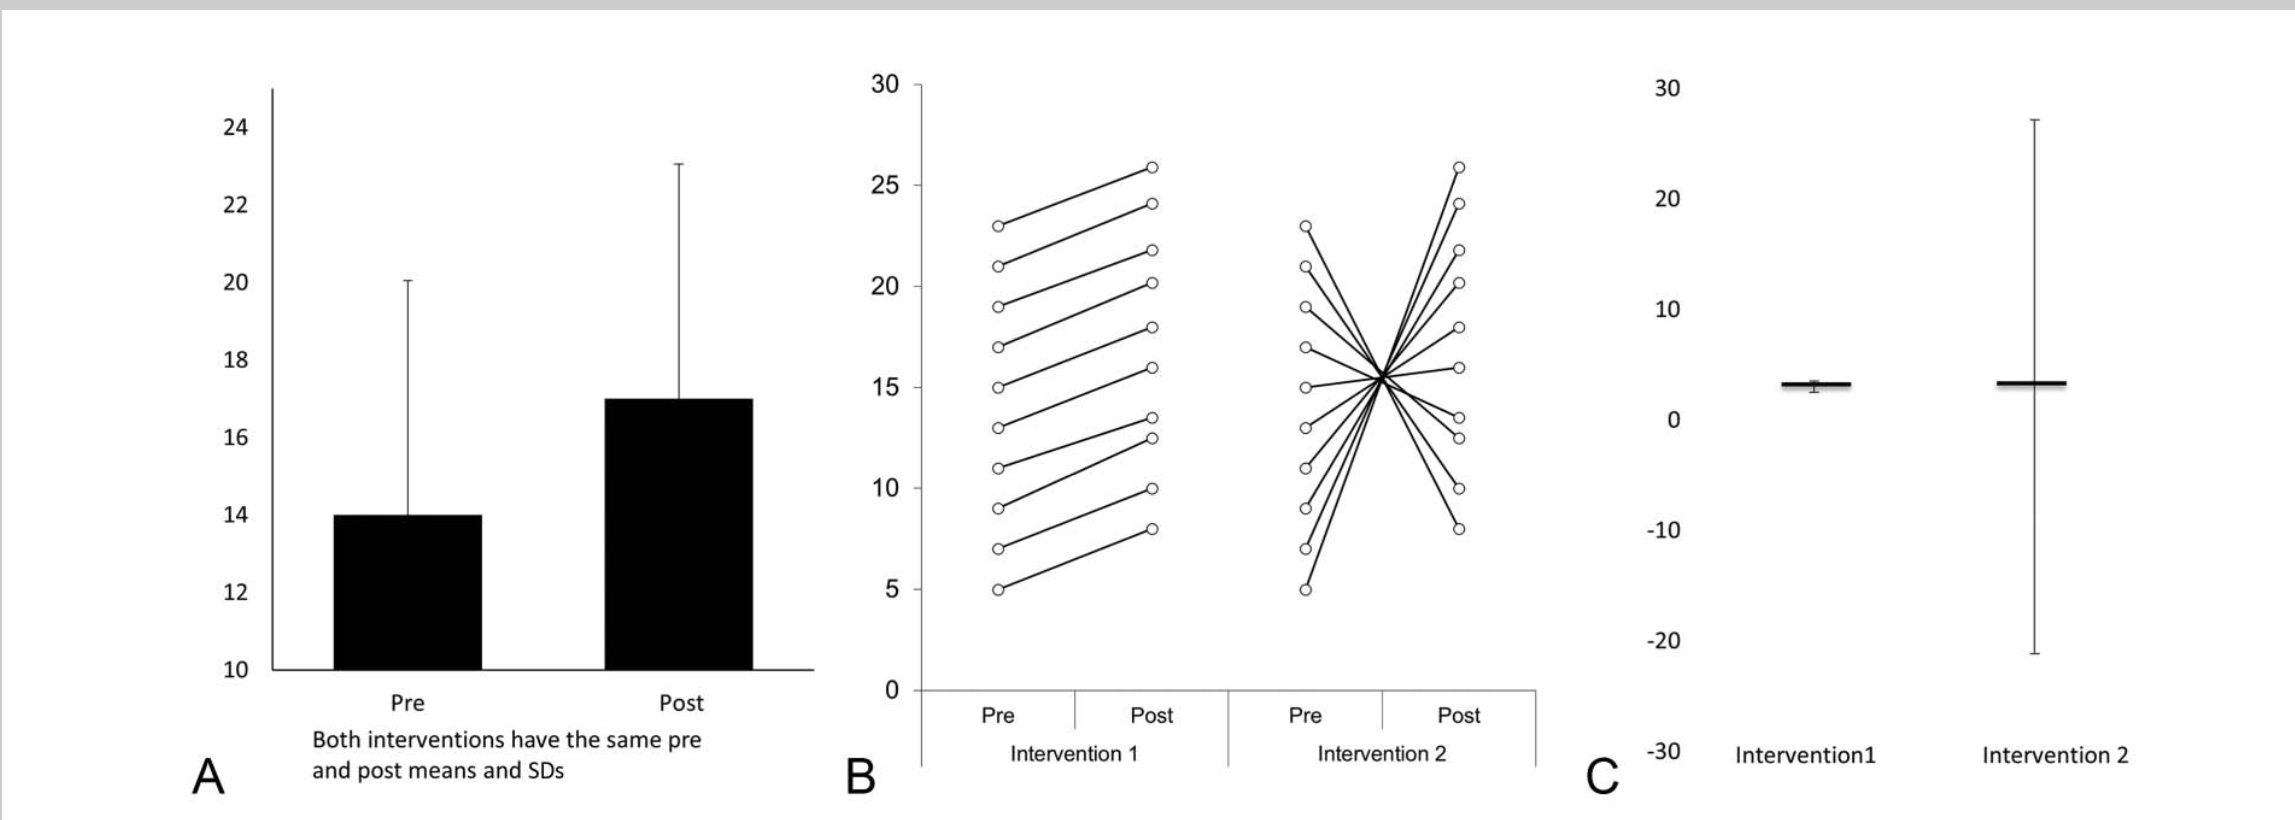
\includegraphics[width=0.75\textwidth]{fig1.png}
\end{figure}
\end{frame}

\begin{frame}{Figure 2}
\protect\hypertarget{figure-2-1}{}
Graph A shows that each intervention has the same pre and post mean but
different pre-post standard deviations. Graph B shows the graph between
pre and post, outlining the same correlations but different pre/post
variabilities, and Graph 3 illustrates the variability further by
showing that the intervention variability is the same. Supports Aim 2.

\begin{figure}[h]
    \centering
    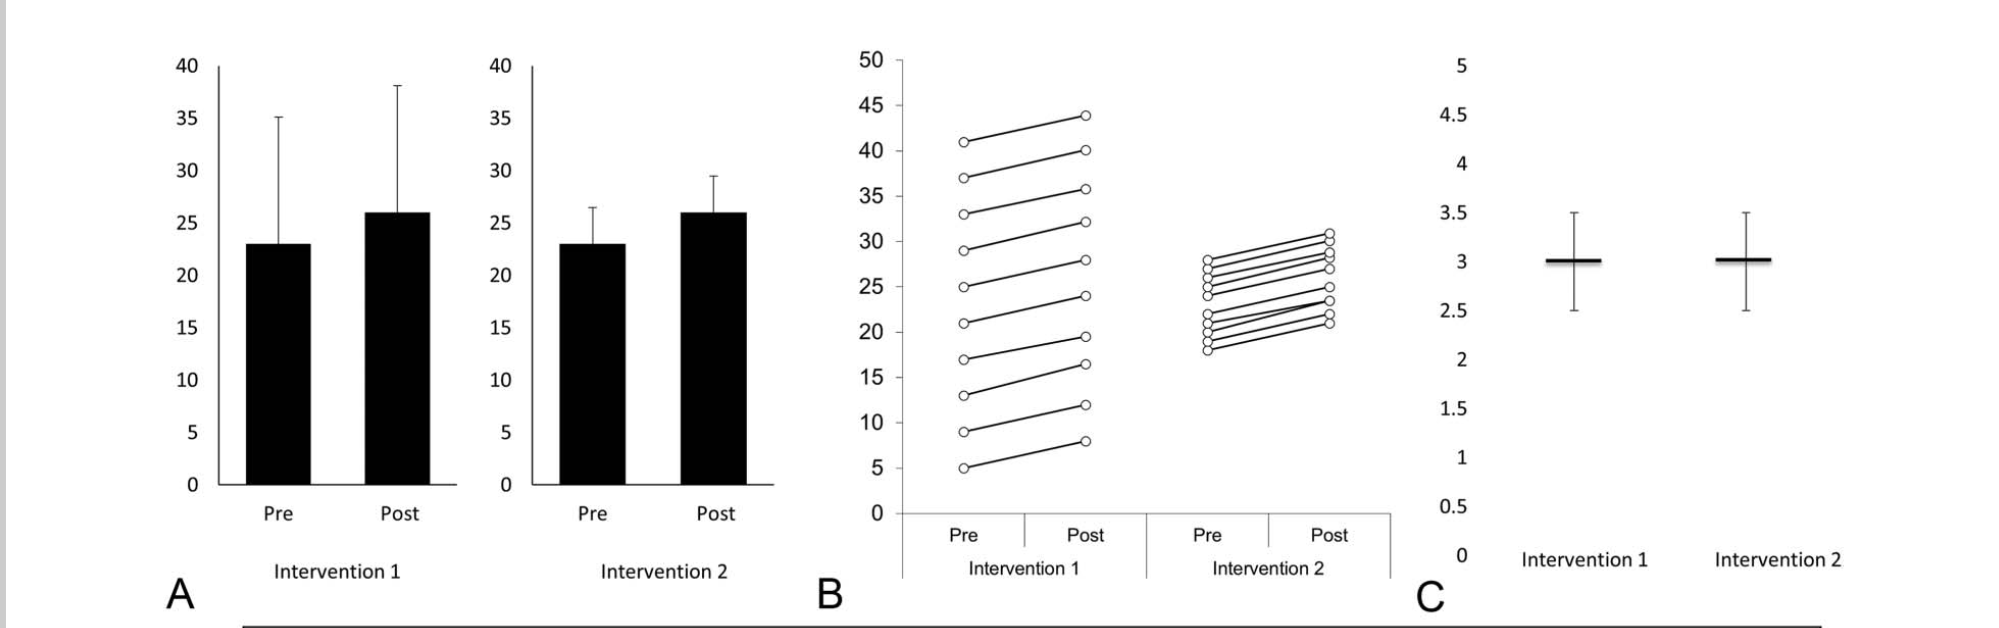
\includegraphics[width=0.75\textwidth]{fig2.png}
\end{figure}
\end{frame}

\begin{frame}{Results (Dankel et. al)}
\protect\hypertarget{results-dankel-et.-al}{}
\begin{figure}[h]
    \centering
    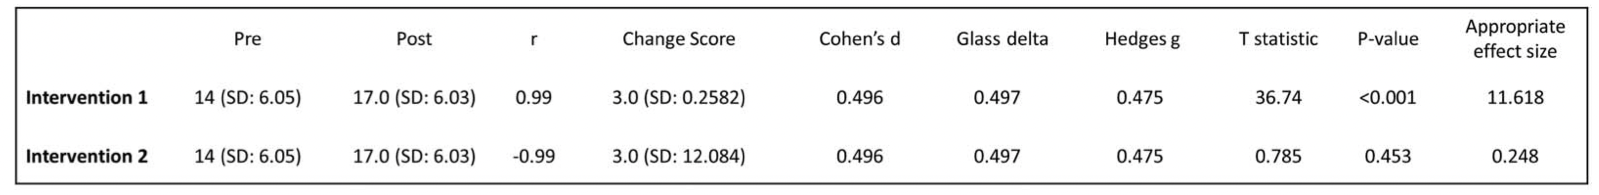
\includegraphics[width=0.75\textwidth]{figresult1.png}
\end{figure}

\begin{figure}[h]
    \centering
    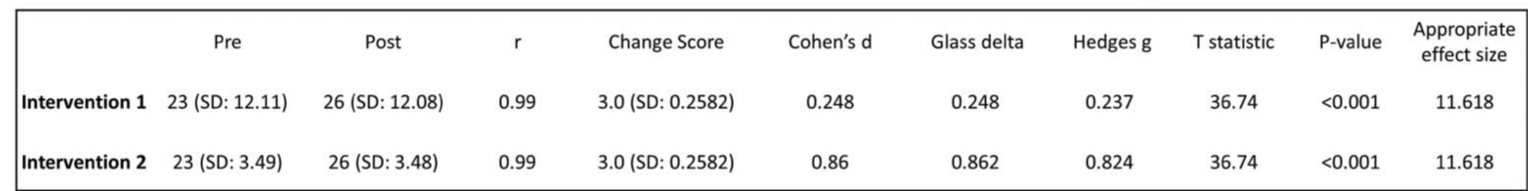
\includegraphics[width=0.75\textwidth]{figresult2.png}
\end{figure}

\begin{itemize}
\tightlist
\item
  Respective to the figures above
\item
  Top attempted to prove aim 1
\item
  Bottom attempted to prove aim 2
\item
  In both, 11.618 is mentioned as the ``Appropriate effect size'' even
  though effect sizes rarely range over 4.
\item
  Standard Deviation of the change scores is suspiciously low as well
\end{itemize}
\end{frame}

\begin{frame}{My Results}
\protect\hypertarget{my-results}{}
mention:
\(SD_\text{change}`=\sqrt{SD_{\text{pre}}^2+SD_{\text{post}}^2-2rSD_{pre}SD_{post}}\)
this is the formula used in the article
\end{frame}

\begin{frame}{Discussion}
\protect\hypertarget{discussion}{}
\begin{block}{General}
\protect\hypertarget{general}{}
Impossible to quantify variability of actual intervention when using
pre-post scores

Figure 1: Intervention 1 produces positive effect where intervention two
does not

Common effect size measures are reliant on the heterogeneity of the
study population

Figure 2 shows identical results in 2 diff groups with the only
difference being that intervention 1 used a more heterogeneous
population
\end{block}

\begin{block}{Other Issues/Notes}
\protect\hypertarget{other-issuesnotes}{}
Notes: normalizing using the preSD only is dependent on the subjects
recruited rather than effectiveness

Also used in triangulation when trying to obtain sample size
calculations
\end{block}
\end{frame}

\begin{frame}{}
\protect\hypertarget{section}{}
\begin{figure}
\centering

\includegraphics[width=0.75\textwidth]{any-questions.jpeg}
\end{figure}

({``Any Questions Image,''} n.d.)
\end{frame}

\begin{frame}{References}
\protect\hypertarget{references}{}
\hypertarget{refs}{}
\begin{CSLReferences}{1}{0}
\leavevmode\vadjust pre{\hypertarget{ref-anyquest}{}}%
{``Any Questions Image.''} n.d. Webpage.
\url{https://mavink.com/explore/Images-for-Any-Questions}.

\leavevmode\vadjust pre{\hypertarget{ref-dankeleffect}{}}%
Dankel, Scott J., and Jeremy P. Loenneke. 2021. {``EFFECT SIZES FOR
PAIRED DATA SHOULD USE THE CHANGE SCORE VARIABILITY RATHER THAN THE PRE-
TEST VARIABILITY.''} \emph{Journal of Strength and Conditioning
Research} 6 (35): 1773--78.

\leavevmode\vadjust pre{\hypertarget{ref-dankelintro}{}}%
Lab, Scott J. Dankel. 2024. {``About Dr. Dankel.''}
\url{https://research.rowan.edu/research-areas/hes/dankel/about.html}.

\leavevmode\vadjust pre{\hypertarget{ref-loennekeintro}{}}%
Ole Miss, Jeremy Paul Loenneke Lab at. 2024. {``Jeremy Paul Loenneke
Introduction.''}
\url{https://hesrm.olemiss.edu/people/jeremy-paul-loenneke/}.

\end{CSLReferences}
\end{frame}

\end{document}
